\newpage
\section{Progettazione e Implementazione}
\label{section:implementazione}
\vspace{10 mm}


Per favorire un modello da studiare che permetta di risolvere gli obiettivi descritti 
pocanzi sono state prese le decisioni qui di seguito elencate.

Iniziamo con il dire che il social network verrà astratto ad un grafo scale-free dove ogni 
nodo è un utente che possiede alcune caratteristiche.

Per il primo obiettivo verrà posta l'attenzione su due algoritmi per la creazione di grafi che 
formano modelli di rete differenti.

Inizialmente verrà fatto vedere come una notizia viene propagata in un grafo di tipo 
``Preferential Attachment'' suggerito da Barabási e Albert~\cite{biblio:barabasilab_emergence}.

Le simulazioni poi proseguiranno con un altra topologia di grafo, sempre scale-free 
con Power Law Degree, descritta però dall'algoritmo di Dorogovtsev e Mendes~\cite{biblio:evolution_networks}.

Il lavoro non parte da dati reali e la scelta di queste topologie di grafi è data 
dalla peculiarità di alcune loro caratteristiche che elencherò qui di seguito:
\begin{itemize}
 \item La topologia di grafo Preferential Attachment:
 \begin{itemize}
  \item è un modello ampiamente utilizzato per la sua semplicità;
  \item è impiegato da buona parte di studi che trattano argomenti somiglianti lo ``Spreading Rumors'';
  \item non è un grafo di tipo frattale~\cite{biblio:fractal_resistant_disease} ma ha una caratteristica simile. 
 Non possedendo cricche di almeno 3 nodi, se un nodo non condivide la notizia, 
 tutti i suoi nodi ``figli'' non riceveranno mai l'informazione e perciò rimarranno per sempre ignoranti sulla notizia.
 \end{itemize}
 
 \item La topologia di grafo definita da Dorogovtsev e Mendes invece:
  \begin{itemize}
  \item ha un modello decisamente più complesso;
  \item può avere all'interno del grafo cricche da 3 o più nodi e questo permette una probabilità maggiore di condivisione della notizia;
  \item più somigliante\footnote{\scriptsize Non esiste un modello virtuale di una rete sociale reale. 
  Tutte le ottimizzazioni che vengono apportate sono per rendere i risultati di queste simulazioni più attinenti alla realtà.}
  ad una struttura reale di rete sociale.
 \end{itemize}
\end{itemize}

Cercando di migliorare il modello totale della simulazione è stato deciso di fornire alcune proprietà alla notizia e 
agli utenti(Nodi) che compaiono nella rete sociale.

Osservando il secondo obiettivo dobbiamo fornire alla notizia un ``argomento'' e per fare ciò si 
è optato per l'inserimento di $N$ valori che definiranno quanto è adatta la notizia per ogni fascia d'età.

Avendo a disposizione la distribuzione delle età, precedentemente mostrata nel grafico di figura~\ref{img:age_distribution_social},
possiamo notare 5 intervalli di anni e quindi stabilire il valore di $N = 5$.
\newpage
Dobbiamo perciò anche definire 5 gruppi di utenti per distinguere le differenti età.
Il numero di persone appartenenti ad ogni gruppo verrà semplicemente definito dalla semplice proporzione:
\begin{equation*}
N\_NODI\_TOTALI \quad / \quad 100 \quad * \quad \%\_UTENTI\_GRUPPO
\end{equation*}
dove $\%\_UTENTI\_GRUPPO$ è la percentuale presente nel grafico di figura ~\ref{img:age_distribution_social}.

A questo punto per la condivisione dell'informazione tra nodo e nodo manca solamente la formula per definire la probabilità 
della propagazione.
Se dovessimo lasciare così le cose avremo un valore della notizia per cui il gruppo condivide ed un altro 
valore per cui non la condivide.
L'idea però è quella di dare la ``possibilità'' all'utente, come nella realtà, di decidere se la 
notizia gli interessa oppure no. 
Questo ci obbliga ad aggiungere un nuovo paramentro all'utente, l'astensione alla notizia.

Così facendo la notizia verrà condivisa dall'utente \emph{'i'} con una certa età \emph{'e'} se:
\begin{equation*}
\Rightarrow NOTIZIA_e \quad > \quad UTENTE_i.astensione
\end{equation*}
dove $\quad NOTIZIA_e \quad$ è la forza di condivisione della notizia su una data fascia d'età \emph{'e'}, 
mentre $\quad UTENTE_i.astensione \quad$ è l'astensione alla notizia dell'utente i-esimo.

L'ultimo obiettivo agisce proprio su quest'ultima parte appena definita.
Quando si parla di ``forza della notizia'' e di ``forza di astensione'' vogliamo considerare un numero tra 0 e 1.
Per avere una probabilità di condivisione più o meno alta andremo ad agire solo sulla ``forza di astensione''.
Per come abbiamo definito la formula della condivisione basterà che la distribuzione dell'astensione sia più 
tendente a 0 per avere una miglior condivisione, o viceversa, più tendente a 1 per avere una peggior
condivisione.

\vspace{5 mm}
\subsection{Strumenti}
\vspace{3 mm}


Dopo aver discusso di tutte le fasi della progettazione possiamo passare all'imple-mentazione.

Le simulazioni previste saranno sviluppate in NetLogo che fornisce un ambiente semplice e piuttosto 
personalizzabile dove si possono condurre studi in parecchi campi.
NetLogo è uno strumento di sviluppo per una programmazione basata ad agenti.
Nel lavoro qui presentato gli agenti in questione saranno gli utenti della rete sociale.

Esistono molti altri simulatori di reti che prevedono una programmazione ad agenti, ma NetLogo
ha risposto brillantemente alle esigenze implementative avendo una sintassi semplice e una moltitudine di
API~\cite{biblio:netlogo_dictionary} fornite dal linguaggio stesso.


\subsection{Topologie dei grafi}
\label{section:graph_topologies}
\vspace{3 mm}


Come già annunciato all'inizio di questo capitolo i modelli di grafo che verranno studiati in questo lavoro
sono due.


\subsubsection{Preferential Attachment}
Il modello Preferential Attachment, come già comunicato a inizio capitolo, è altamente diffuso e conosciuto.
Tanto da avere una propria API per la creazione nel dizionario di NetLogo.

Invocando la funzione:
\begin{lstlisting}[label=some-code, style=custom_code]
 generate-preferential-attachment turtles links num-nodes
\end{lstlisting}

che risiede all'interno dell'estensione ``network'' verrà creato un grafo di num-nodes con le proprietà 
del grafo Preferential Attachment.\\
In figura \ref{img:preferential_attachment} è presente una rappresentazione grafica del grafo.


\subsubsection{Modello di Dorogovtsev e Mendes}
Il modello definito da Dorogovtsev e Mendes viene implementato dalla libreria Java chiamata GraphStream~\cite{biblio:graphstream}.
La libreria è formata essenzialmente da tre parti: 
\begin{itemize}
 \item core: Il package principale di GraphStream;
 \item algo: Il package dove sono implementati tutti gli algoritmi e i generatori della libreria;
 \item ui: Il package che permette di visualizzare e dare un layout al grafo.
\end{itemize}
I grafi che verranno utilizzati nelle simulazioni sono stati creati da un'applicazione implementata appositamente.
Una volta creati vengono salvati su file in formato GraphML~\cite{biblio:graphml} per poter 
essere caricati dalla simulazione NetLogo. 
Nella figura~\ref{img:gui_main} si può notare il pulsante per importare il file GraphML.\\
In figura \ref{img:dorogovtsev_mendes} è presente una rappresentazione grafica del grafo.

\begin{figure}[!ht]
 \centerline{
  \begin{subfigure}[b]{0.42\textwidth}
    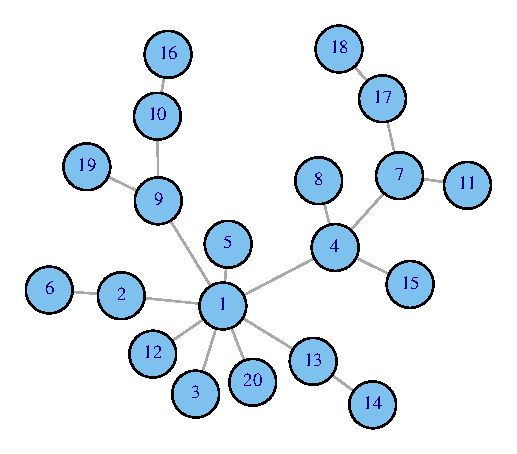
\includegraphics[width=1.0\textwidth]{img/preferential-attachment-graph.eps}
    \caption{Preferential Attachment}
    \label{img:preferential_attachment}
  \end{subfigure}
  \qquad
  \qquad
  \begin{subfigure}[b]{0.42\textwidth}
    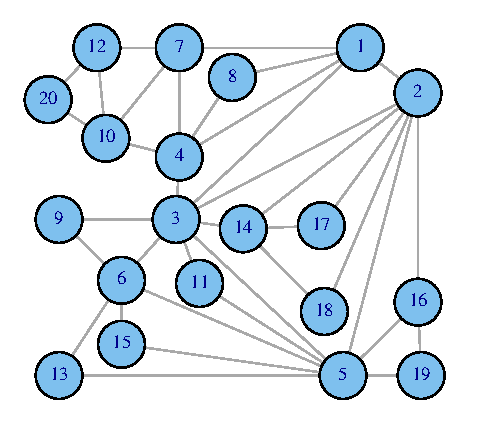
\includegraphics[width=1.0\textwidth]{img/dorogovtsev-mendes-graph.eps}
    \caption{Dorogovtsev e Mendes}
    \label{img:dorogovtsev_mendes}
  \end{subfigure}
 }
 \caption{Rappresentazione grafica delle due topologie di grafo studiate.}
 \label{img:graph_models}
\end{figure}




\subsection{Interfaccia grafica per la configurazione della rete}
\label{section:gui_setup_graph}
\vspace{3 mm}

\begin{wrapfigure}{r}{0.37\textwidth}
  \vspace{-40pt}
  \begin{center}
    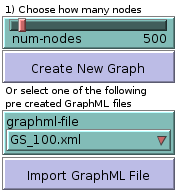
\includegraphics[width=0.30\textwidth]{img/gui-graph.png}
  \end{center}
 \vspace{-10pt}
 \caption{GUI per la creazione/importazione del grafo}
 \vspace{-10pt}
 \label{img:gui_graph}
\end{wrapfigure}
Al fine di portare a termine gli obiettivi in precedenza descritti è stato necessario importare nel progetto, 
dal grafico di figura~\ref{img:age_distribution_social}, i dati di alcuni Social Netwoks.


\begin{wrapfigure}{l}{0.37\textwidth}
  \vspace{-20pt}
  \begin{center}
    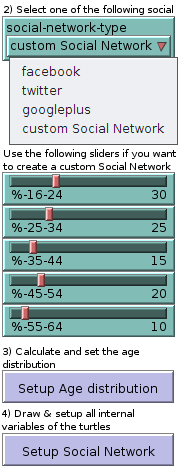
\includegraphics[width=0.30\textwidth]{img/gui-main.png}
  \end{center}
 \vspace{-10pt}
 \caption{GUI principale: 
 scelta del Social Netwoks;
 pulsante per il calcolo della distribuzione delle età;
 pulsante per l'inizializzazione dei nodi.}
 \vspace{-10pt}
 \label{img:gui_main}
\end{wrapfigure}

Sono stati selezionati solo i tre che seguono per via della loro popolarità:
\begin{itemize}
 \item Facebook
 \item Twitter
 \item Google+
\end{itemize}

Per rendere l'applicazione più generale possibile sono stati implementati anche 5 cursori che permettono di far 
decidere all'utilizzatore dei parametri personalizzati e che per semplicità intuitiva sono 
stati chiamati:\\ ``\%-<fascia età inizio>-<fascia età fine>.
Si può vedere la loro implementazione in figura~\ref{img:gui_main}.



L'ultimo obiettivo, invece, servirà ad analizzare un'interazione tra 2 diversi gruppi di utenti, che 
permetterà di studiare il numero di visualizzazioni della notizia in casi più complessi.
Un esempio potrebbe essere quello di voler dividere il numero totale delle persone in due sottoinsiemi così formati
L'ultimo obiettivo, invece, servirà ad analizzare un'interazione tra 2 diversi gruppi di utenti, che 
permetterà di studiare il numero di visualizzazioni della notizia in casi più complessi.
Un esempio potrebbe essere quello di voler dividere il numero totale delle persone in due sottoinsiemi così formati
L'ultimo obiettivo, invece, servirà ad analizzare un'interazione tra 2 diversi gruppi di utenti, che 
permetterà di studiare il numero di visualizzazioni della notizia in casi più complessi.
Un esempio potrebbe essere quello di voler dividere il numero totale delle persone in due sottoinsiemi così formati
L'ultimo obiettivo, invece, servirà ad analizzare un'interazione tra 2 diversi gruppi di utenti, che 
permetterà di studiare il numero di visualizzazioni della notizia in casi più complessi.
Un esempio potrebbe essere quello di voler dividere il numero totale delle persone in due sottoinsiemi così formati
L'ultimo obiettivo, invece, servirà ad analizzare un'interazione tra 2 diversi gruppi di utenti, che 
permetterà di studiare il numero di visualizzazioni della notizia in casi più complessi.
Un esempio potrebbe essere quello di voler dividere il numero totale delle persone in due sottoinsiemi così formati










